%no borrar PREAMBULO
\documentclass[12pt]{article}

\usepackage[top=3.5 cm, bottom=2.5  cm, left=3 cm, right=3 cm]{geometry}
\usepackage{fancyhdr}
\pagestyle{fancy}

\usepackage[hidelinks]{hyperref} %esta opción saca las cajas de colores de los hiperlinks

\fancyfoot[C]{\thepage }  %numera las páginas

\usepackage[utf8]{inputenc}

\usepackage{amsmath,amsfonts,amssymb}
\usepackage{xcolor}
\usepackage{fancyvrb}
\newcommand\verbbf[1]{\textcolor[rgb]{0,0,1}}%comando para colorear el texto en verbatim

%\linespread{1} %por si queremos achicar el espacio entre lineas

\usepackage{tabularx,booktabs}
\usepackage{graphicx}
\usepackage{float} %para que las figuras puedan ponerse en cualquier lado

\usepackage{subcaption}
\usepackage{layout}
\usepackage{multicol}  %para escribir en columnnas 
\usepackage{float}
\usepackage{textcomp}
\usepackage{natbib}
\usepackage{tikz}
\usepackage{multirow} %para cambiar el alto de una fila en una tabla
\tikzset{
  connect/.style = { dashed, gray }
}
\usepackage{pgfplots}
\pgfplotsset{compat=1.8}
\usepackage[english ,spanish]{babel}
\usepackage{latexsym}
\usepackage{verbatim}

%\usepackage{alltt}
\usepackage{indentfirst}

\usepackage[flushmargin]{footmisc} %para alinear las notas de página

\usepackage{url}
\usepackage{advdate}
\usepackage{wrapfig}
\usepackage{amsthm}
\usepackage[inline]{enumitem} %para hacer listas en una linea, los mismos comandos con *
\newtheorem*{myteo}{Teorema} % la * es para no numerarlos
\newtheorem*{myexample}{Ejemplo}
\newtheorem*{myprop}{Proposición}
\newtheorem*{mylem}{Lema}
\theoremstyle{definition}
\newtheorem*{mydef}{Definición}
\newtheorem{ejer}{Ejercicio}
\newtheorem*{mydefs}{Definiciones}
\theoremstyle{remark}
\newtheorem*{myobs}{Observación}


\renewcommand{\baselinestretch}{1}  %interlineado

\addto\captionsspanish{%
  \renewcommand{\figurename}{Figura}%
}

\newcommand\myText[1]{\text{\scriptsize\tabular[t]{@{}l@{}}#1\endtabular}}
\addto\captionsspanish{%
  \renewcommand{\tablename}{Tabla}%
}

\def \ds {\displaystyle} %define un comando abreviado  
\def\com{“R”}

\usepackage{hyperref}%para referencias de internet con link!
\newcommand*{\fullref}[1]{\hyperref[{#1}]{ \nameref*{#1}}}
%comando \fullref para que ademas del número de capitulo, sección etc. escriba el título del capitulo, sección o lo que sea a lo que estamos haciendo referencia

\newcommand\comentario[1]{\textcolor{red}{#1}}%comentarios en el pdf

\interfootnotelinepenalty=10000 %previene que se pasen a otra página las notas de pie
\raggedbottom 
\addtolength{\topskip}{0pt plus 10pt}
\addtolength{\footnotesep}{0.1mm}

\VerbatimFootnotes%para poder usar Verbatim en las notas de pie

\begin{document}

\fancyhf{}
\pagestyle{fancy}
\lhead{Departamento de Matem\'{a}tica\\Universidad Nacional del Comahue}
\rhead{Matem\'{a}tica 1\\ Licenciatura en Ciencias Biol\'{o}gicas}

%HASTA ACA 

\begin{centering}
\Large{\textbf{Trabajo Práctico N° 3}}\\
\large{\textbf{Lógica y Conjuntos}}\\
\end{centering}
\begin{enumerate}
%1
\item Determinar si las siguientes expresiones son proposiciones y cuáles no lo son. Explicar por qué.
\begin{multicols}{2}
 \begin{itemize}
 \setlength\itemsep{0em}
        \item El sol es cuadrado.
        \item La cuchara sirve para.
        \item La mamá sirve postre.
        \item Mi bisabuela se peinó con rodete el 16 de julio de 1899.
        \item ¿Qué hora es?
        \item ¿Existe la justicia?
        \item Existe la justicia
        \item No existe la justicia
        \item $2 + 5 = 6$
        \item $2 + 5 = 7$
        \item$2 + 5 $
  \end{itemize}
\end{multicols}

%2
\item En el lenguaje común, hay varias expresiones que se utilizan indistintamente para la misma forma lógica.  Por ejemplo:
 \begin{multicols}{2}
 \begin{itemize}
 \setlength\itemsep{0em}
    \item Algunos mamíferos tienen alas. 
   	\item Nadie es perfecto.
	\item Cualquier  múltiplo de 6 puede dividirse por 3. 
	\item Todos los insectos alados tienen 6 patas. 
	\item No hay mamíferos acuáticos. 
	\item Existen hombres daltónicos.
	\item Unos pancitos tienen queso. 
	\item Hay algunos sitios de acampe donde no se puede hacer fuego.
	\item Las cámaras digitales utilizan baterías.
  \end{itemize}
\end{multicols}

Redactar las proposiciones anteriores en la forma \textit{Todo...} o \textit{Existe...}. Por ejemplo: “Algunos mamíferos tienen alas” se escribirá como “Existe un mamífero que tiene alas”. 

%3
\item Dadas las siguientes proposiciones,
 \begin{multicols}{2}
 \begin{itemize}
 \setlength\itemsep{0em}
     	\item Todos los perros son blancos.
	\item Hay mamíferos que vuelan.
	\item Existe un león que ruge.
	\item Los leones tienen melena.
	\item Hay gallinas que ponen huevos verdes.
	\item Ningún metal es líquido.
	\item Hay plantas que no se reproducen por semillas.
  \end{itemize}
\end{multicols}
 Se pide, identificar un conjunto de referencia para cada uno  y redactar las proposiciones anteriores de la forma  \textit{Todo...} o \textit{Existe...} (cuando sea necesario)(¡no es importante si las afirmaciones son verdaderas o falsas!)

Ejemplo: Todos los perros son blancos $\rightarrow$  \textit{Conjunto de referencia}: El conjunto de todos los perros que existen. \textit{Enunciado en la forma “ Todo…” }  $\rightarrow$ Todo perro es blanco.

%4
\item Proponer algunas proposiciones que incluyan cuantificadores y redactarlas en la forma   \textit{Todo...} o \textit{Existe...}.

%5
\item Explicar cómo demostrarías si las afirmaciones del inciso 2) son verdaderas o falsas.
%6

%7
\item Escribir la negación de las siguientes proposiciones (independientemente de la verdad o falsedad de la afirmación):
\begin{itemize}
\setlength\itemsep{0em}
	\item Existen planetas con agua en el sistema solar.
	\item Ningún alumno ingresante a la universidad debe materias de la escuela secundaria.
	\item Todos los egresados de escuelas secundarias del país hacen su viaje de estudios a Bariloche.
	\item Hay mamíferos acuáticos.
	\item Cualquier miembro de la Asociación Argentina de Ecología tiene descuentos en los congresos de la misma. 
\end{itemize}

%8
\item Considere un referencial $R$ formado por las siguientes figuras donde hay tres formas (triángulo, cuadrado y círculo), en dos tamaños (grande y pequeño) y  tres “colores” (negro, blanco y a rayas) que se muestran en la página siguiente. Tenemos $18$ formas posibles que surgen de combinar las características forma, tamaño y color.  Ahora llamemos:
\begin{itemize}
\item A al conjunto de todas las figuras del referencial que hagan verdadera la proposición \textbf{n}: “la figura es negra”
\item B al conjunto de todas las figuras del referencial que hagan verdadera la proposición \textbf{g}: “la figura es grande” 
\end{itemize}
\begin{figure}[H]
\centering
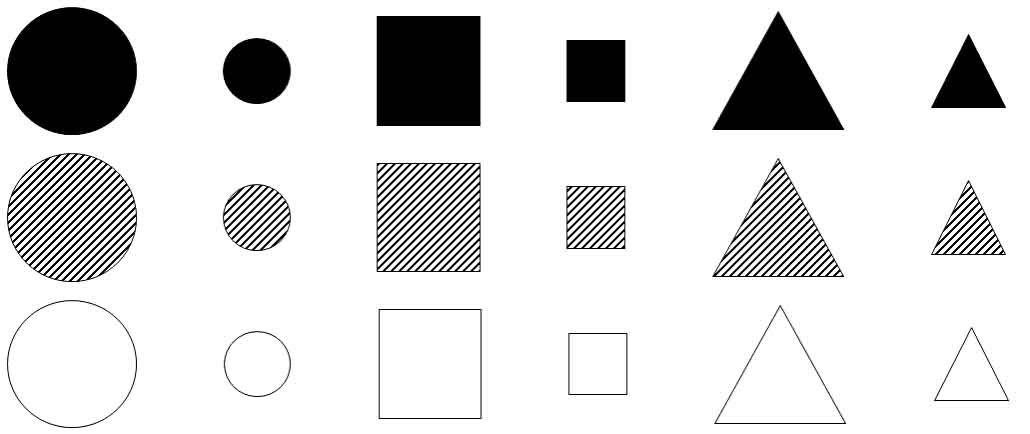
\includegraphics[width=0.7\textwidth]{tp3_fig1}
\caption{Conjunto referencial. Las figuras se clasifican por forma, color y tamaño}
\end{figure}
\begin{enumerate}
\item Representar gráficamente los conjuntos A y B mediante un diagrama de Venn como el siguiente: 
\begin{figure}[H]
\centering
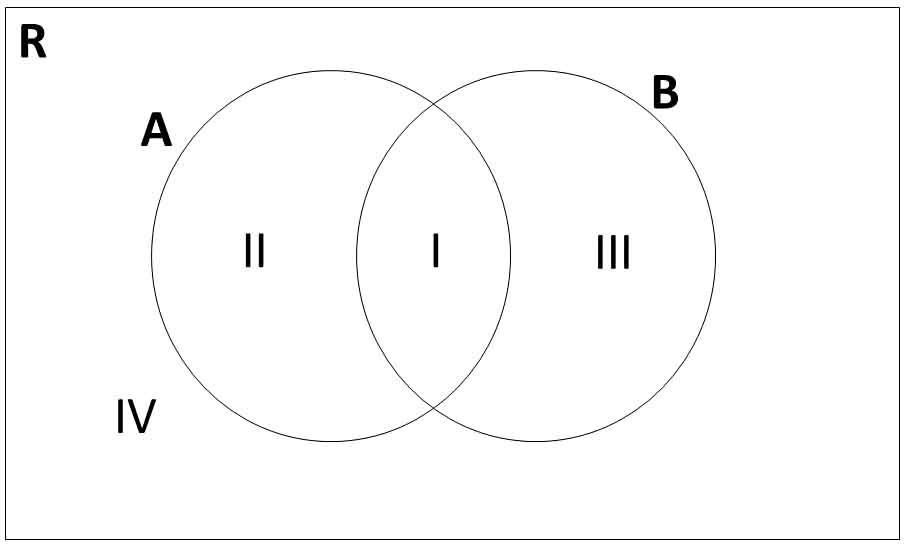
\includegraphics[width=0.5\textwidth]{tp3_fig2}
\end{figure}
\item De acuerdo a esta representación, ¿qué elementos se encuentran en la región $A\cap B$?
\item Enunciar la proposición compuesta que verifican los elementos de $A\cap B$ utilizando el conectivo lógico $\wedge$.
\item ¿Qué elementos se encontrarán en la región II? Escribir la proposición compuesta con el conectivo correspondiente.
\item ¿Qué elementos se encontrarán en la región III? Escribir la proposición compuesta con el conectivo correspondiente.
\item ¿Qué elementos se encontrarán en la región IV? Escribir la proposición compuesta con el conectivo correspondiente.
\end{enumerate}

%9
\item Para el mismo referencial del ejercicio anterior, supongamos ahora que:
\begin{itemize}
\setlength\itemsep{0em}
\item A es conjunto de todas las figuras del referencial que hacen verdadera la proposición \textbf{b}: “la figura es blanca”.
\item B es conjunto de todas las figuras del referencial que hacen verdadera la proposición \textbf{t}: “la figura es triángulo”. 
\end{itemize}
Si representamos gráficamente estos conjuntos mediante un diagrama de Venn como en el caso anterior:

\begin{enumerate}
\item Enunciar, haciendo uso de conectivos lógicos, las proposiciones que hacen verdaderas las figuras que se ubican en las regiones  I, II, III y IV.\\
\item Describir las figuras del referencial R que se ubican en la unión de A y B. Enunciar la proposición compuesta que cumplen los elementos de  $A\cup B$ utilizando el conectivo lógico  $\vee$.\\
\item Si una figura no es triángulo pero está en $A\cup B$, ¿qué podemos afirmar de esa figura?\\
\item Escribir algunas proposiciones compuestas utilizando el conectivo “o inclusivo” ($\vee$) y el “o excluyente” ($\veebar$) y analizar en qué casos serán verdaderas.\\
\end{enumerate}

%10
\item En el lenguaje matemático, ¿es correcto decir “3 es menor o igual que 5”? y ¿es correcto decir  “5 es menor o igual que 5”?

%11
\item En una librería aparece escrito: “Nuestros clientes en posesión de constancia de alumno regular o de empleado de la Universidad tendrán derecho al $15\%$ de descuento”. ¿Quiénes obtienen el descuento?

%12
\item Llamemos R a un conjunto referencial cualquiera, $A$ al conjunto de los elementos de R que hacen verdadera la proposición \textbf{p} y $B$ al conjunto de los elementos de R que hacen verdadera la proposición \textbf{q}. Completar el siguiente cuadro:

\begin{table}[ H]
\begin{center} 
\begin{tabular} { l c c l }
\textbf{Proposición}&\textbf{Forma conjuntista}& & \textbf{Representación gráfica}\\ \hline  \\ 
%\hline
\textbf{p} es Verdadera& A& & \begin{minipage}{5cm} \begin{center} 
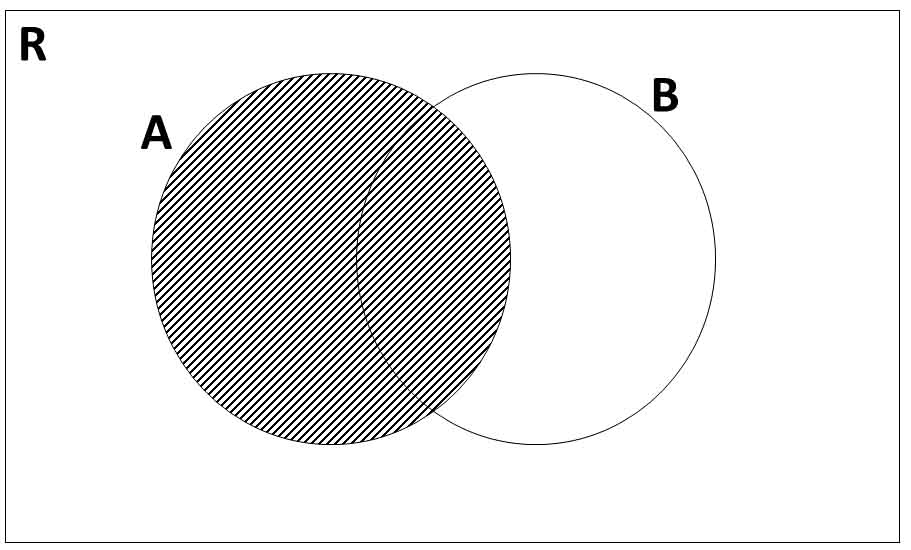
\includegraphics[width=0.6\textwidth]{tp3_fig3} 
\end{center}
\end{minipage}\\ \\ 
$..........................$&$\bar{A}$ & & \begin{minipage}{5cm}  \begin{center} 
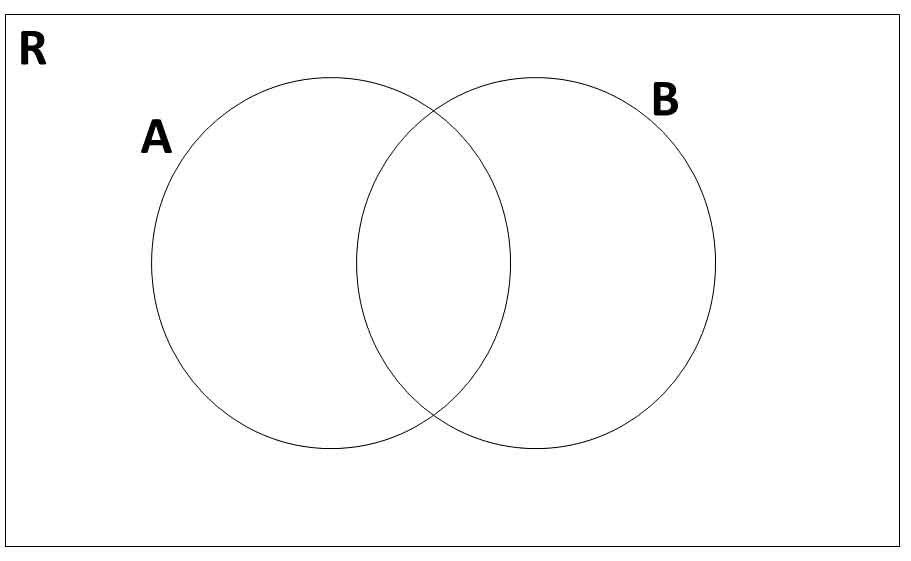
\includegraphics[width=0.6\textwidth]{tp3_fig6} 
\end{center}
\end{minipage}\\ \\   
$..........................$&$..........................$ & & \begin{minipage}{5cm} \begin{center} 
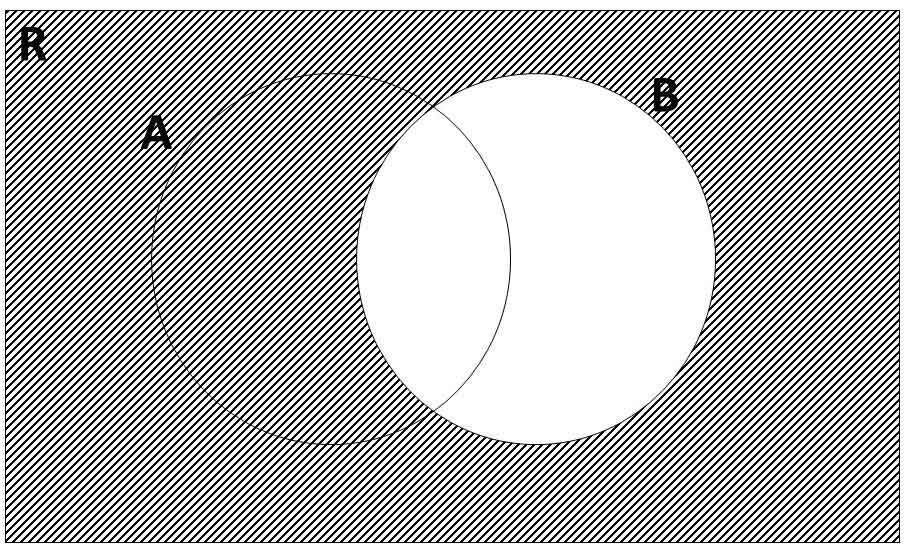
\includegraphics[width=0.6\textwidth]{tp3_fig4} 
\end{center}
\end{minipage}\\ \\ 
 $p \wedge q$ es verdadera&$..........................$ & &\begin{minipage}{5cm} \begin{center} 
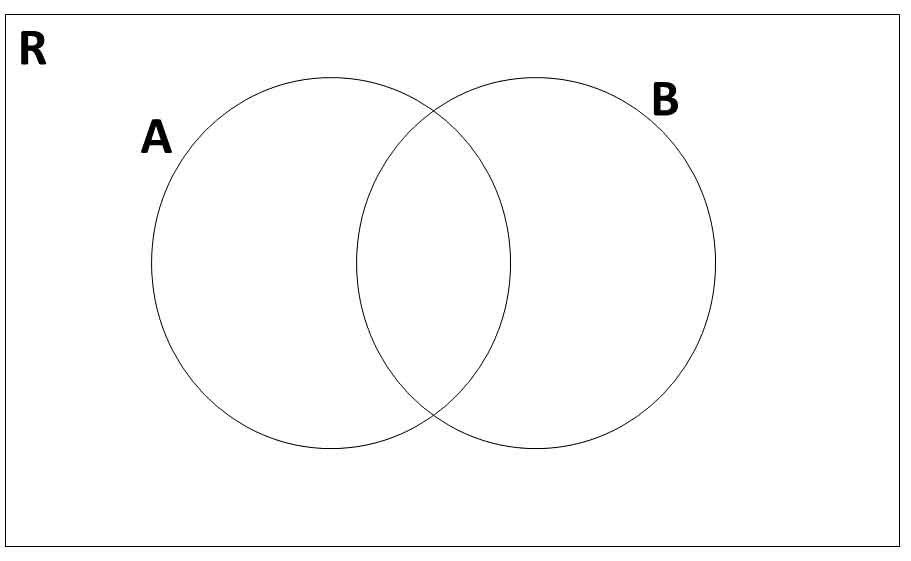
\includegraphics[width=0.6\textwidth]{tp3_fig6} 
\end{center}
\end{minipage}\\ \\  
$..........................$&$\bar{A}\cup \bar{B} = \overline{A\cap B}$ & & \begin{minipage}{5cm} \begin{center} 
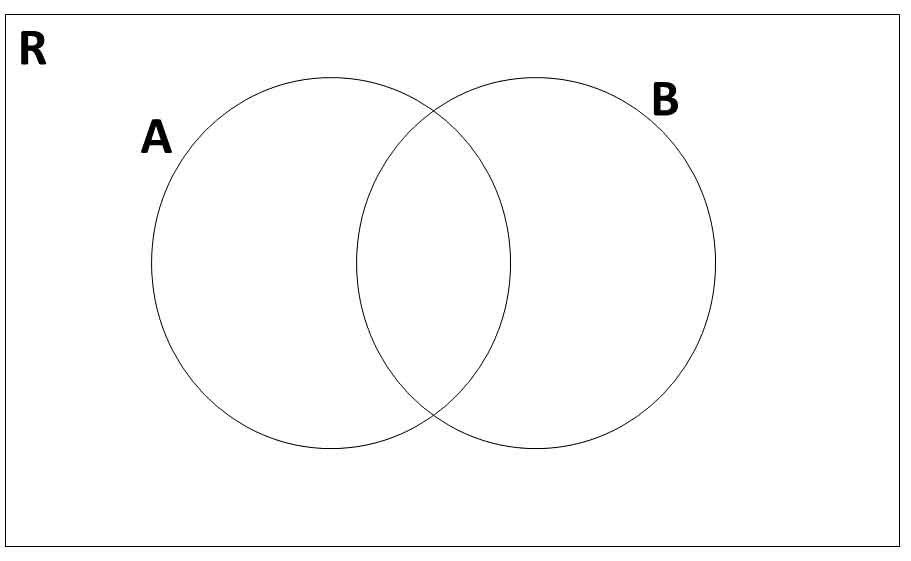
\includegraphics[width=0.6\textwidth]{tp3_fig6} 
\end{center}
\end{minipage}\\ \\

\end{tabular} 
\end{center} 
\end{table}

\begin{table}[ H]
\begin{center} 
\begin{tabular} { l c c l }
\textbf{Proposición}&\textbf{Forma conjuntista}& & \textbf{Representación gráfica}\\ \hline  \\ 
%\hline
  
$..........................$&$..........................$ & & \begin{minipage}{5cm} \begin{center} 
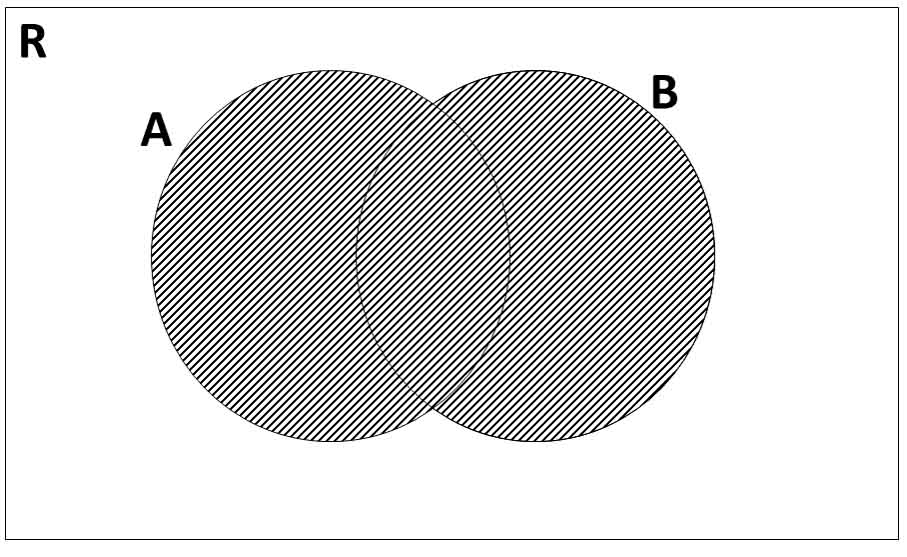
\includegraphics[width=0.6\textwidth]{tp3_fig5} 
\end{center}
\end{minipage}\\ \\ 
 $p \vee q$ es falsa& $..........................$& & \begin{minipage}{5cm} \begin{center} 
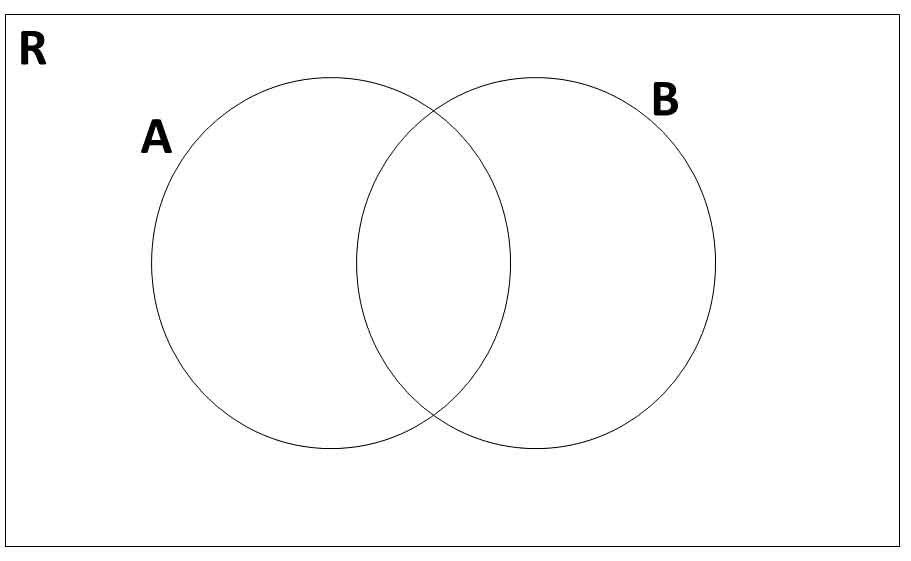
\includegraphics[width=0.6\textwidth]{tp3_fig6} 
\end{center}
\end{minipage}\\ \\   
$..........................$&$..........................$ & & \begin{minipage}{5cm} \begin{center} 
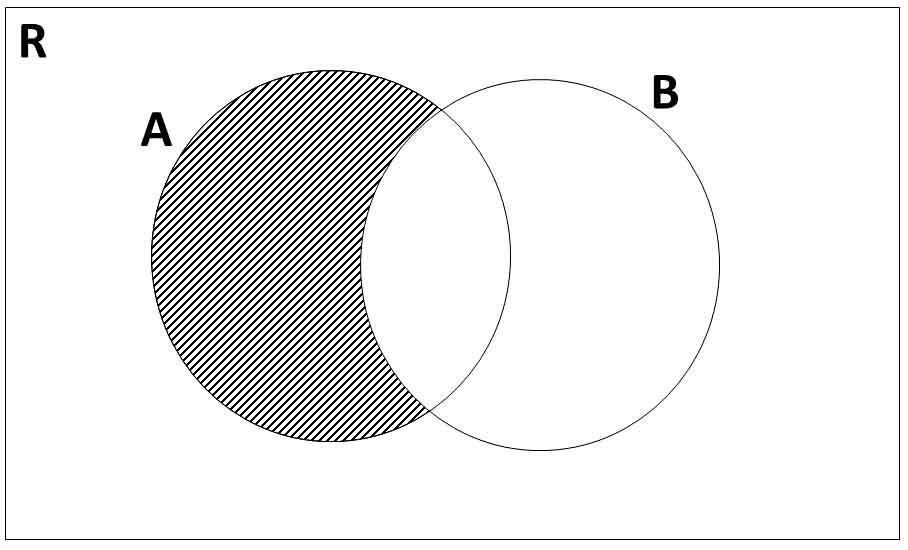
\includegraphics[width=0.6\textwidth]{tp3_fig7} 
\end{center}
\end{minipage}\\ \\   
$..........................$&$..........................$ & & \begin{minipage}{5cm} \begin{center} 
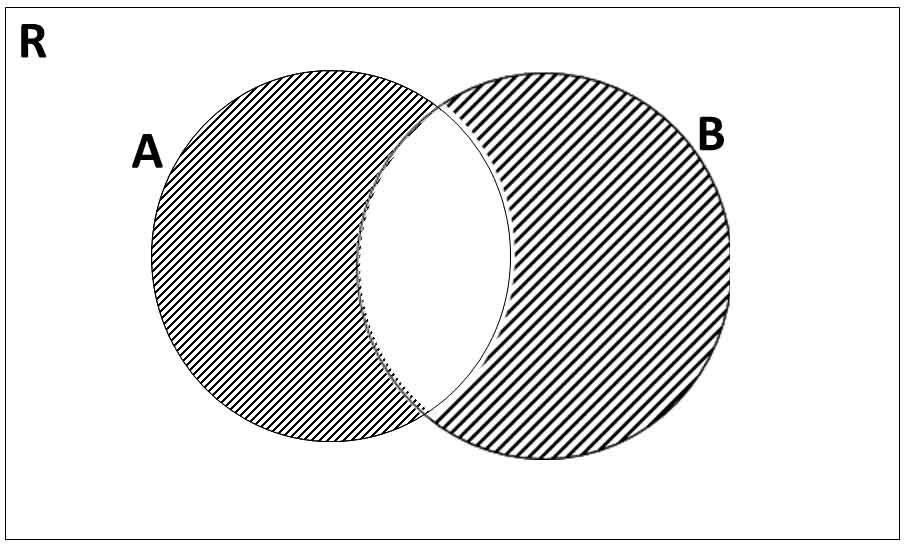
\includegraphics[width=0.6\textwidth]{tp3_fig8} 
\end{center}
\end{minipage}
\end{tabular} 
\end{center} 
\end{table}

%13
\item Considerar el conjunto  $T = \{0, 1, 2, 3, 4, 5, 6, 7, 8, 9, 10, 11, 12, 13, 14, 15, 16\}$ y las siguientes proposiciones:
\begin{itemize}
\setlength\itemsep{0em}
\item \textbf{p} es la proposición abierta: $x$ es un número par,
\item \textbf{q} es la proposición abierta: $x$ es un número de una cifra,
\item \textbf{r} es la proposición abierta: $x$ es un número divisible por 3.
\end{itemize}
Escribir el enunciado de las siguientes proposiciones  compuestas y los conjuntos resultantes:
$p \vee q$,  $p \wedge q$, $p \wedge q  \wedge r$ y $ q \wedge \sim r$

%19
\item Consideremos los siguientes ejemplos:
\begin{itemize}
\setlength\itemsep{0em}
\item Es suficiente que un número sea múltiplo de 8 para que sea divisible por 2.
\item Es suficiente nacer en Argentina para ser sudamericano.
\item Es suficiente cargar 70 litros de nafta para llegar desde Bariloche hasta El Bolsón (aprox. 120 km).
\item Es suficiente fotosintetizar para ser vegetal.
\end{itemize}
¿Qué significado tiene que una condición sea suficiente para que se cumpla otra? 

%20
\item En los enunciados anteriores, reconocer el antecedente y el consecuente y escribirlos como una implicación.

%21
\item Enunciar algunos condicionales donde el antecedente sea una condición suficiente para que ocurra el consecuente. Escribirlos en lenguaje coloquial y como una implicación.

%22
\item Consideremos ahora las siguientes proposiciones:
\begin{itemize}
\setlength\itemsep{0em}
\item Para ser investigador de Conicet es necesario haber alcanzado el grado de doctor.
\item Es necesario ser mayor de edad para emitir un voto electoral.
\item Es necesario ser mamífero para ser ballena.
\item Es necesario estar inscripto en la carrera Licenciatura en Ciencias Biológicas para cursar Matemática 1 como alumno regular.
\end{itemize}
¿Qué significado tiene que una condición sea necesaria para que se cumpla otra? 

%23
\item En los enunciados anteriores, reconocer el antecedente y el consecuente y escribirlos como una implicación.

%28
\item Vimos que las expresiones siguientes son equivalentes: 
\begin{itemize}
\setlength\itemsep{0em}
\item \textbf{Si} p \textbf{entonces} q.
\item \textbf{Todo} p \textbf{es} q (todo x que verifica p verifica q).
\item \textbf{p} $\Rightarrow$ \textbf{q}.
\item p es \textbf{condición suficiente} para q.
\item q es \textbf{condición necesaria} para p.
\end{itemize}
Por ejemplo, consideremos las proposiciones \textbf{p}: el animal x es una ballena y \textbf{q}: el animal x es un mamífero. El condicional  \textit{Si un animal  es una ballena, entonces es un mamífero} se puede escribir en forma equivalente de las siguientes maneras:
\begin{itemize}
\setlength\itemsep{0em}
\item \textbf{Todo} p \textbf{es} q $\rightarrow$ {Toda} ballena \textbf{es} mamífero.
\item \textbf{p} $\Rightarrow$ \textbf{q} $\rightarrow$  ser ballena implica ser mamífero $\rightarrow$  ballena $\Rightarrow$ mamífero.
\item p es \textbf{condición suficiente} para q $\rightarrow$  ser ballena es \textbf{condición suficiente} para ser mamífero.
\item q es \textbf{condición necesaria} para p $\rightarrow$  ser mamífero es \textbf{condición necesaria} para ser ballena.
\end{itemize}
Enunciar una proposición condicional verdadera y escribirla de estas cinco formas equivalentes.

%24
\item  Enunciar algunos condicionales donde esté involucrada una condición necesaria entre el antecedente y el consecuente. Escribirlos en lenguaje coloquial y como una implicación.

%25
\item ¿Siempre una condición suficiente es necesaria? Mostrar ejemplos.

%26
\item ¿Siempre una condición necesaria es suficiente? Mostrar ejemplos.

%27
\item Considerar la proposición: “Para que una figura sea un triángulo es necesario y suficiente que tenga tres lados”. ¿Qué significado tiene que una condición sea necesaria y suficiente para que se cumpla otra? 


%29
\item Enunciar una proposición condicional verdadera en la que se  utilice el cuantificador \textit{todo} y escribirla de las cinco formas propuestas en el ítem anterior.\\

\textbf{Algunos problemas adicionales sobre proposiciones condicionales}

%14
\item \label{primerAviso} Concentremos la atención en aquellas implicaciones que aparecen “ocultas” en el lenguaje coloquial. Consideremos el siguiente ejemplo publicado en un diario:
 
\textit{ “Para cargo gerencial se busca Licenciado en Ciencias Económicas, con referencias comprobables de al menos dos empresas en el ramo, menor de 40 años, con posibilidades de radicarse en la ciudad de Neuquén”.}

Reconocé las proposiciones (simples o compuestas) que forman el antecedente y el consecuente y escribí el aviso en un enunciado de la forma \textit{Si... entonces...} utilizando los conectivos que necesites.

%15
\item Escribir en la forma \textit{Si... entonces...}, el siguiente aviso publicado en el diario (es un diario de mentira):

\textit{Becas de ayuda económica para estudiantes del interior. La Provincia de Río Negro beneficiará con becas de ayuda económica a estudiantes egresados de colegios secundarios de la provincia que se inscriban en carreras de más de dos años de duración en Universidades Nacionales, cuyos padres no superen en conjunto un ingreso de $\$1500$ en concepto de salarios y constituyan un grupo familiar de más de $5$ personas}.

%16
\item Cuestiones para pensar en relación a estos dos avisos, para el caso en que las implicaciones sean verdaderas. Para el primer aviso (ejercicio \ref{primerAviso}), entre otras, estas dos personas pretenden el trabajo:
\begin{itemize}
\item Juan Gómez, Licenciado en Ciencias Económicas, casado, de 43 años de edad con amplia experiencia en empresas del ramo, podría radicarse en Neuquén.
\item Pablo Ramos, Licenciado en Ciencias Económicas y Analista de Sistemas, de 33 años de edad, presenta seis cartas de recomendación de empresas en el ramo, residente en Neuquén. 
\end{itemize}
\begin{enumerate}
\setlength\itemsep{0em}
\item Juan Gómez ¿puede aspirar al cargo? ¿Por qué?
\item Pablo Ramos ¿puede aspirar al cargo? ¿Por qué?
\item ¿Pablo Ramos obtendrá el cargo?
\item Si le dieron a José Ulloa el cargo, ¿qué sabemos de él? (Supongamos que no hay acomodo).
\end{enumerate}
 
%17
\item Para el segundo aviso (siempre cumpliendo la ley):
\begin{enumerate}
\setlength\itemsep{0em}
\item Proponer ejemplos hipotéticos de estudiantes que pueden obtener la beca y de estudiantes que no podrían. Explicar. 
\item Si a Marcela García le dieron la beca, ¿qué sabemos de ella?
\item Si a Rosa González no le dieron la beca, ¿qué sabemos de ella?
\end{enumerate}

%18
\item \label{permisoConducir} Escribir el siguiente enunciado en la forma  \textit{Si... entonces...} usando proposiciones compuestas y los conectivos 
necesarios:

\textit{Para obtener el permiso de conducir, debés cumplimentar los siguientes requisitos:
\begin{itemize}
\setlength\itemsep{0em}
\item tener 18 años cumplidos, 
\item presentar certificados de salud psicofísica,
\item saber manejar,
\item pagar una prima de $\$350$,
\item aprobar un examen de manejo en la municipalidad local.
\end{itemize}}

\begin{enumerate}
\setlength\itemsep{0em}
\item No obtuviste tu permiso: ¿qué pudo pasar?
\item Lo obtuviste: ¿qué pasó necesariamente?
\end{enumerate}


%30
\item Pensemos de nuevo el ejemplo del permiso de conducir (ejercicio \ref{permisoConducir}), pero ahora suponiendo que se cumple la ley a rajatabla. ¿Sería verdadera la implicación recíproca? ¿Por qué? 
 
%% agregar problemas de afirmaciones recíprocas

\end{enumerate}
%\pagebreak
\noindent
\textbf{Problemas de repaso}

\begin{enumerate} 
%1
\item  Considerar los siguientes subconjuntos de los números naturales (sin incluir al cero):
\begin{itemize}
\setlength\itemsep{0em}
\item A: conjunto de los números pares.
\item B: conjunto de los múltiplos de 8.
\item C: conjunto de números terminados en 0.	
\item D: conjunto de los números primos mayores que 10.
\item E: conjunto de los múltiplos de 3. 
\item F: conjunto de los números de una cifra. 
\end{itemize}

\begin{enumerate}
\setlength\itemsep{0em}
\item Indicar un referencial y ubicar en un diagrama los conjuntos A, B, C, D, E, y F.
\item Escribir las proposiciones que hacen verdaderas los elementos de:\\
 \begin{enumerate}
     \item $A \cap C \cap E$
     \item $A\cap D$
     \item $B -  E$
\end{enumerate}
\item Escribir una implicación verdadera (de la forma: \textit{Si... entonces...}) en relación a las proposiciones que hacen verdaderas los elementos de los conjuntos definidos.
\item En relación a los conjuntos propuestos, escribir una proposición verdadera que contenga el cuantificador \textit{todo} y otra que contenga el cuantificador \textit{existe}.
\item Expresar la negación lógica de las dos afirmaciones escritas en el inciso anterior (obviamente falsas).
\end{enumerate}

%2
\item  Considerar los siguientes conjuntos personas que caminan por el CRUB (referencial):
\begin{itemize}
\setlength\itemsep{0em}
\item A: conjunto de personas cuyo apellido empieza con A.
\item B: conjunto de personas que cursan materias de primer año.
\item C: conjunto de alumnos de la Licenciatura en Biología. 
\item D: conjunto de alumnos de cuarto año de la Licenciatura en Biología.
\item E: conjunto de personas de apellido Gómez.
\item F: conjunto de personas de apellido Álvarez.
\end{itemize}
\begin{enumerate}
\setlength\itemsep{0em}
\item Representar estos conjuntos usando diagramas de Venn.
\item En cada región determinada por los conjuntos ubicar ejemplos (inventados).
\item Escribir las proposiciones que hacen verdaderas los elementos de:
 \begin{enumerate}
     \item $A \cap B$
     \item $A\cup C$
     \item $B -  A$
     \item $\bar{A}$
\end{enumerate}
\item Escribir una implicación verdadera (de la forma: “Si...entonces...”) en relación a las proposiciones que hacen verdaderas los elementos de los conjuntos definidos.
\item Escribir una afirmación verdadera que contenga el cuantificador \textit{todo} y otra que contenga el cuantificador \textit{existe} (en relación a los conjuntos propuestos).
\item Expresar la negación lógica de las dos afirmaciones escritas en el inciso anterior (obviamente falsas).
\end{enumerate}

%3
\item \textbf{La lógica y las reglas ortográficas de acentuación}\\
\\Consideremos las siguientes definiciones y reglas ortográficas del lenguaje castellano, donde no tendremos en consideración las excepciones (que siempre existen) a las mismas:\\
\\
\textbf{Definiciones}:
\begin{itemize}
\setlength\itemsep{0em}
\item \textbf{Acento}: es la mayor intensidad con que se pronuncia una sílaba en la pronunciación de una palabra (por ejemplo “palabra” está acentuada en la segunda sílaba, y matemática en la tercera).
\item \textbf{Acento prosódico}: es el acento que se pronuncia pero no se escribe. Por ejemplo la palabra “tuberculosis” tiene acento prosódico en la cuarta sílaba. 
\item \textbf{Acento gráfico} o \textbf{tilde}: es el acento que se pronuncia y se escribe. Por ejemplo la palabra “espíritu” tiene tilde en la segunda sílaba.
\item \textbf{Palabras agudas}: son las palabras acentuadas en la última sílaba (camión, carril).
\item \textbf{Palabras graves}: son las palabras acentuadas en la penúltima sílaba (cabeza, revólver). 
\item \textbf{Palabras esdrújulas}: son las acentuadas en la antepenúltima sílaba o anteriores (matemática, últimamente).
\end{itemize}

\textbf{Reglas}: Palabras que llevan acento gráfico o tilde:
\begin{itemize}
\setlength\itemsep{0em}
\item Regla 1: Las palabras agudas terminadas en \textit{n}, \textit{s} o \textit{vocal} llevan tilde.
\item Regla 2: Las palabras graves no terminadas en \textit{n}, \textit{s} o \textit{vocal} llevan tilde.
\item Regla 3: Las palabras esdrújulas siempre llevan tilde sea cual fuera su terminación.   
\end{itemize}

Consideremos ahora los siguientes conjuntos definidos dentro del conjunto referencial de todas las palabras del idioma español:
\begin{itemize}
\setlength\itemsep{0em}
\item A el conjunto formado por las palabras con tilde.
\item B el conjunto formado por las palabras sin tilde.
\item C el conjunto formado por las palabras agudas.
\item D el conjunto formado por las palabras graves.
\item E el conjunto formado por las palabras esdrújulas. 
\item F el conjunto formado por las palabras terminadas en n, s o vocal.
\end{itemize}

\begin{enumerate}
\item Diseñar un diagrama de Venn que muestre la relación entre los conjuntos A, B, C, D y E.

\item Ubicar en ese gráfico las palabras \textit{maní} y \textit{dosel}.

\item Haciendo uso de una proposición compuesta (y utilizando el conectivo adecuado), indicar qué características cumplen los elementos de $B \cap C$. Dar un ejemplo.

\item  Haciendo uso de una proposición compuesta (y utilizando el conectivo adecuado) indicar qué características cumplen los elementos de $D \cap F$. Dar un ejemplo.

\item Cada uno de los conjuntos definidos reúne los elementos del conjunto referencial que verifican una proposición abierta. Por ejemplo los elementos del conjunto A son los que verifican la proposición \textbf{a}: “x es una palabra con tilde”. Así, la palabra \textit{maní} es un elemento del conjunto A (porque la proposición “\textit{maní} es una palabra con tilde” es verdadera), mientras que \textit{calle} no es un elemento del conjunto A (porque la proposición “\textit{calle} es una palabra con tilde” es falsa). Es decir, cada conjunto tiene “asociada” una proposición abierta de manera que todos los elementos del referencial que la hacen verdadera conforman el conjunto. Llamemos con letras minúsculas a las proposiciones que inducen a los conjuntos A hasta F definidos más arriba. Escribir (con palabras) las siguientes proposiciones compuestas:\\
\begin{multicols}{3}
 \begin{enumerate}
\item $d \vee f$ 
\item $e\wedge f$		
\item $\sim e\vee f$
\end{enumerate}
\end{multicols}

\item Escribir una nueva proposición en este contexto tal que ningún elemento la haga verdadera.

\item Mencionar dentro de este contexto todos los casos posibles (a partir de las proposiciones A hasta F) donde tiene sentido conectar las proposiciones con el “o excluyente”.

\item Escribir ejemplos de proposiciones (simples o compuestas) dentro de este contexto que satisfagan las afirmaciones siguientes: 
\begin{itemize}
\item ........................ es condición necesaria (no suficiente) para ........................
\item ........................ es condición suficiente (no necesaria) para ........................
\item ........................ es condición suficiente y necesaria para ...........................
\end{itemize}

\item Deducir si las afirmaciones siguientes son verdaderas o falsas y justificar adecuadamente:
\begin{enumerate}
\item Existen palabras graves sin tilde.
\item Ninguna palabra esdrújula tiene tilde.
\item Existen palabras con tilde que no terminan en n, s o vocal.
\item Toda palabra aguda tiene tilde.
\end{enumerate}

\item  Escribir las negaciones de las afirmaciones del ítem anterior, haciendo uso de los cuantificadores \textit{todo} y \textit{existe}

\item  Completar:
\begin{itemize}
\item $a \wedge c \Rightarrow  ..... $ 
\item $\sim c \wedge \sim d \wedge a \Rightarrow ..... $		 
\end{itemize}

\end{enumerate}


\end{enumerate}

\end{document}
